\chapter{Data cleaning} % Main appendix title

\label{AppendixD}
\label{sec:slewratecleaning}

In 2016 data there was an issue in ECAL pulse reconstruction. A correction to mitigate the effect
was applied to electron and photon objects, but the PF 
candidates, which are inputs to both jets and \ptmiss, are not modified. Instead the correction was propagated to \ptmiss based on \dR\ 
matching of these objects while jets are left unmodified. While most of the events where corrections are not properly propagated are 
rejected by \dphi cuts between leading two jets and \ptmiss directions, a few events still seem to survive after various selections.  To 
account for residual effects of this reconstruction feature on this analysis, $p_{\text{T}}^{jet}$/\ptg $\geq$ 1 where the jet and photon 
are matching within $\dR<0.3$. Since a jet matching to a photon is nothing but the photon candidate clustered with neighboring activities, 
the $p_{\text{T}}^{jet}$ is expected to be higher than \ptg. This is verified to be so in MC with  
$p_{\text{T}}^{jet}$/\ptg as a function of \ptg as shown in Figures~\ref{fig:ratioVsPhotonPt} top-left for 
low-\dphi region with \ptmiss$>$100~\gev and top-right for high-\dphi region with 100$<$\ptmiss$<$200~\gev. The same quantities for these 
event selection show a distinct population in data events as shown in bottom row of Figure~\ref{fig:ratioVsPhotonPt}. 

%Distributions of $p_{\text{T},\gamma}$, $\eta_{\gamma}$, \ptmiss, and $\Delta\phi (\ptmiss,\gamma)$  before and after the $p_{\text{T,jet}}$/$p_{\text{T},\gamma}$ $\geq$ 1 for the events  with high-\dphi and 100\ptmiss$<$200~\gev are shown in Figure~\ref{fig:fixedPhotonAndMET}. Clearly the distributions for these quantities in data are much better behaved and compare well with MC after applying this cleaning. The effect of cleaning is also checked in single electron sample used for background estimation. The distributions of electron \pt is shown before and after this cleaning in data and MC in Figure~\ref{fig:fixed-e-mu-cr} upper panel. The distributions are well behaved and compare better with MC as well as with those of muon \pt in single muon control sample as shown in lower panel.

\begin{figure}[h]
  \centering
  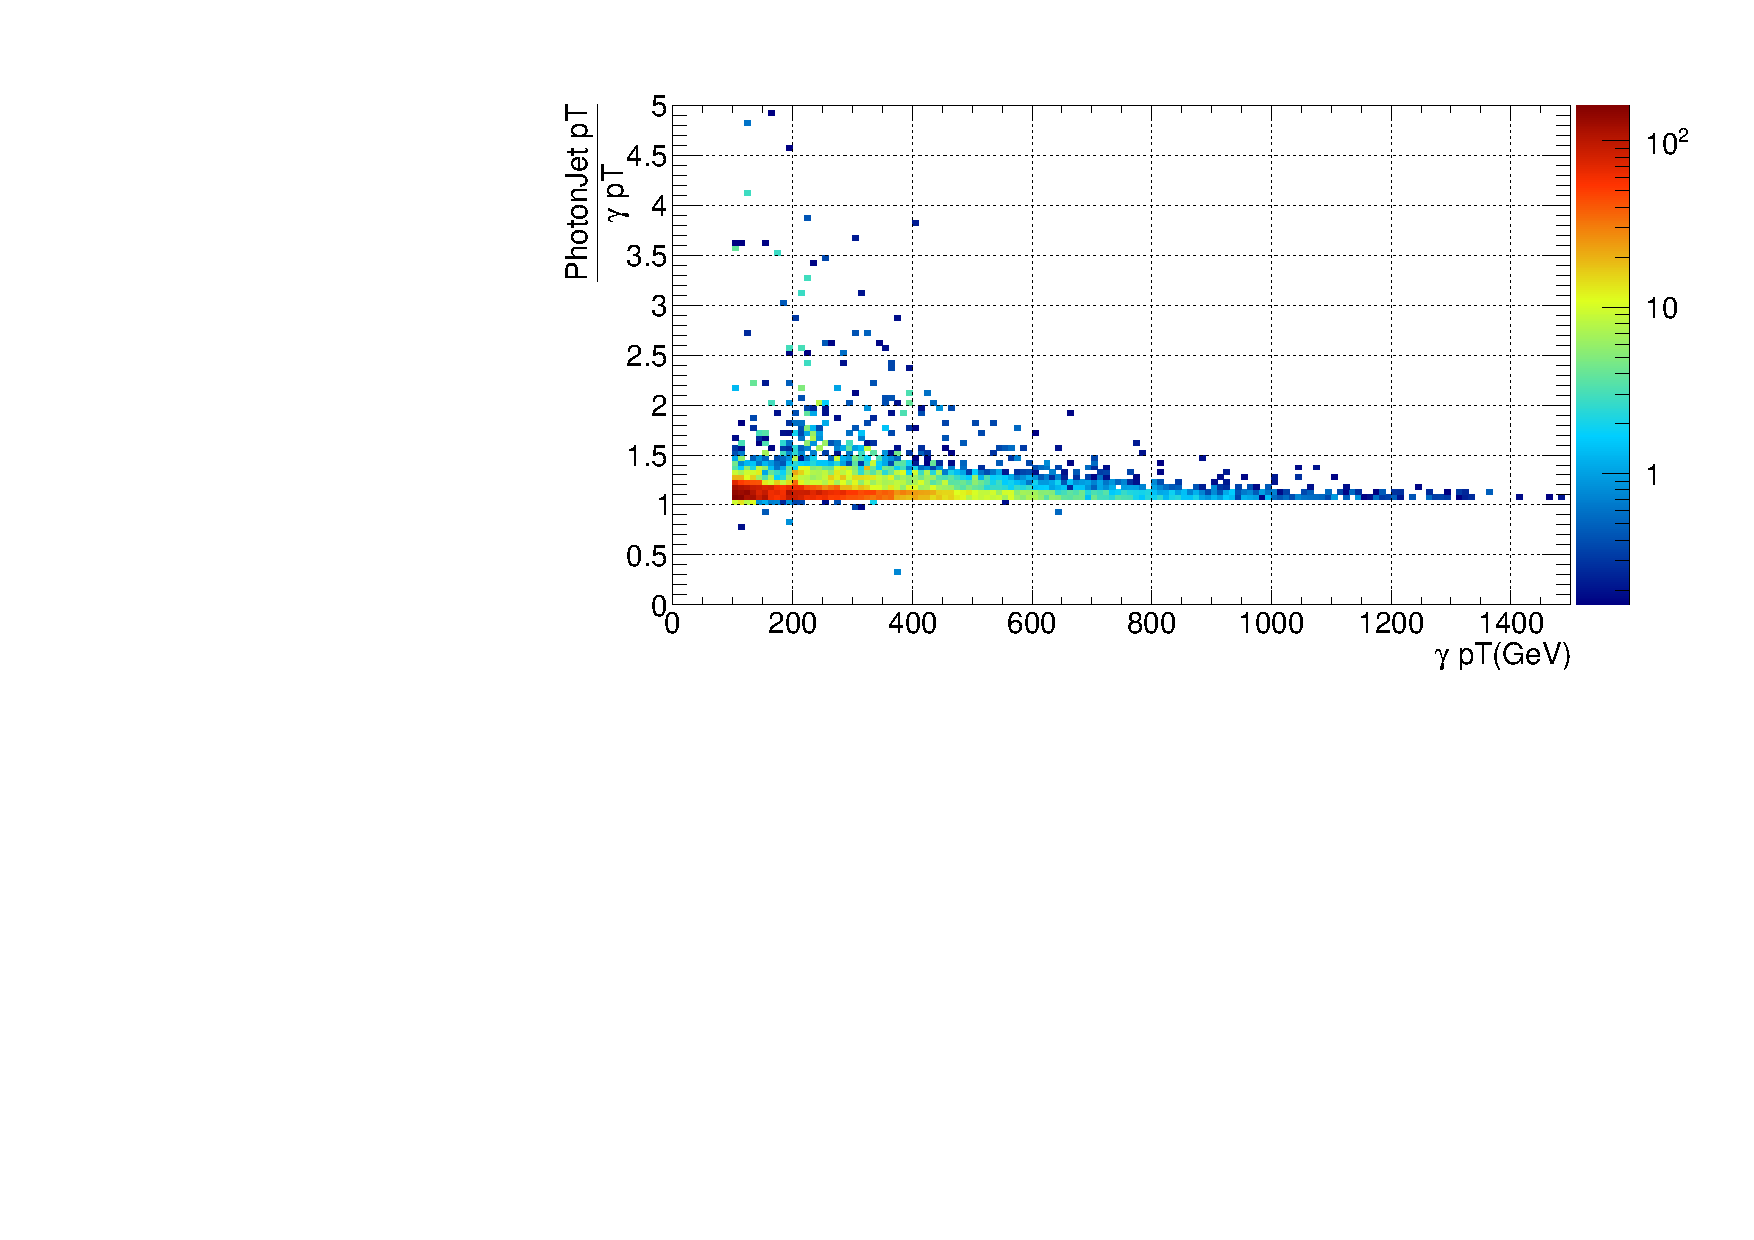
\includegraphics[width=0.48\linewidth]{../Figures/Chap2/appendix/RatioPhoJetPtToPhoPtVsPhoPt_AB_MultijetMC.pdf}
  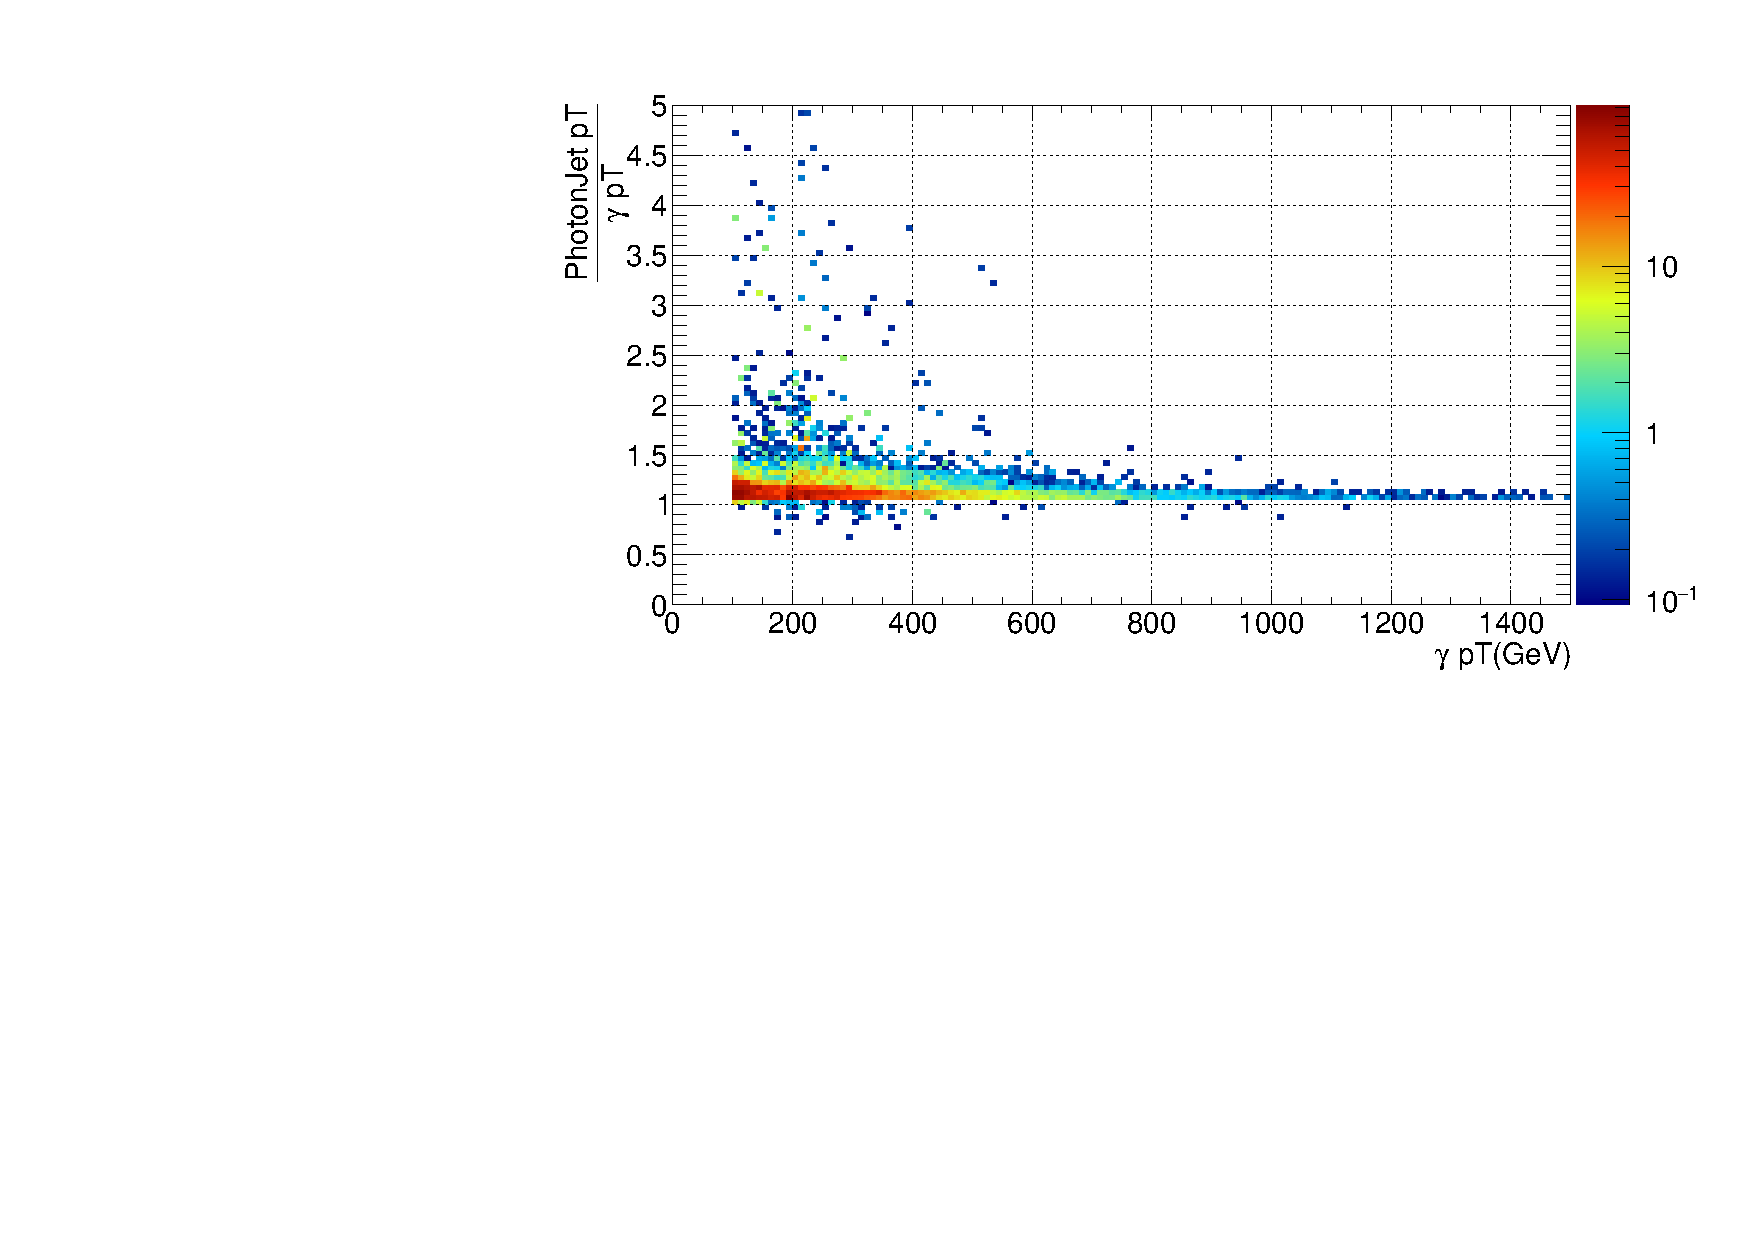
\includegraphics[width=0.48\linewidth]{../Figures/Chap2/appendix/RatioPhoJetPtToPhoPtVsPhoPt_C_MultijetMC.pdf}
  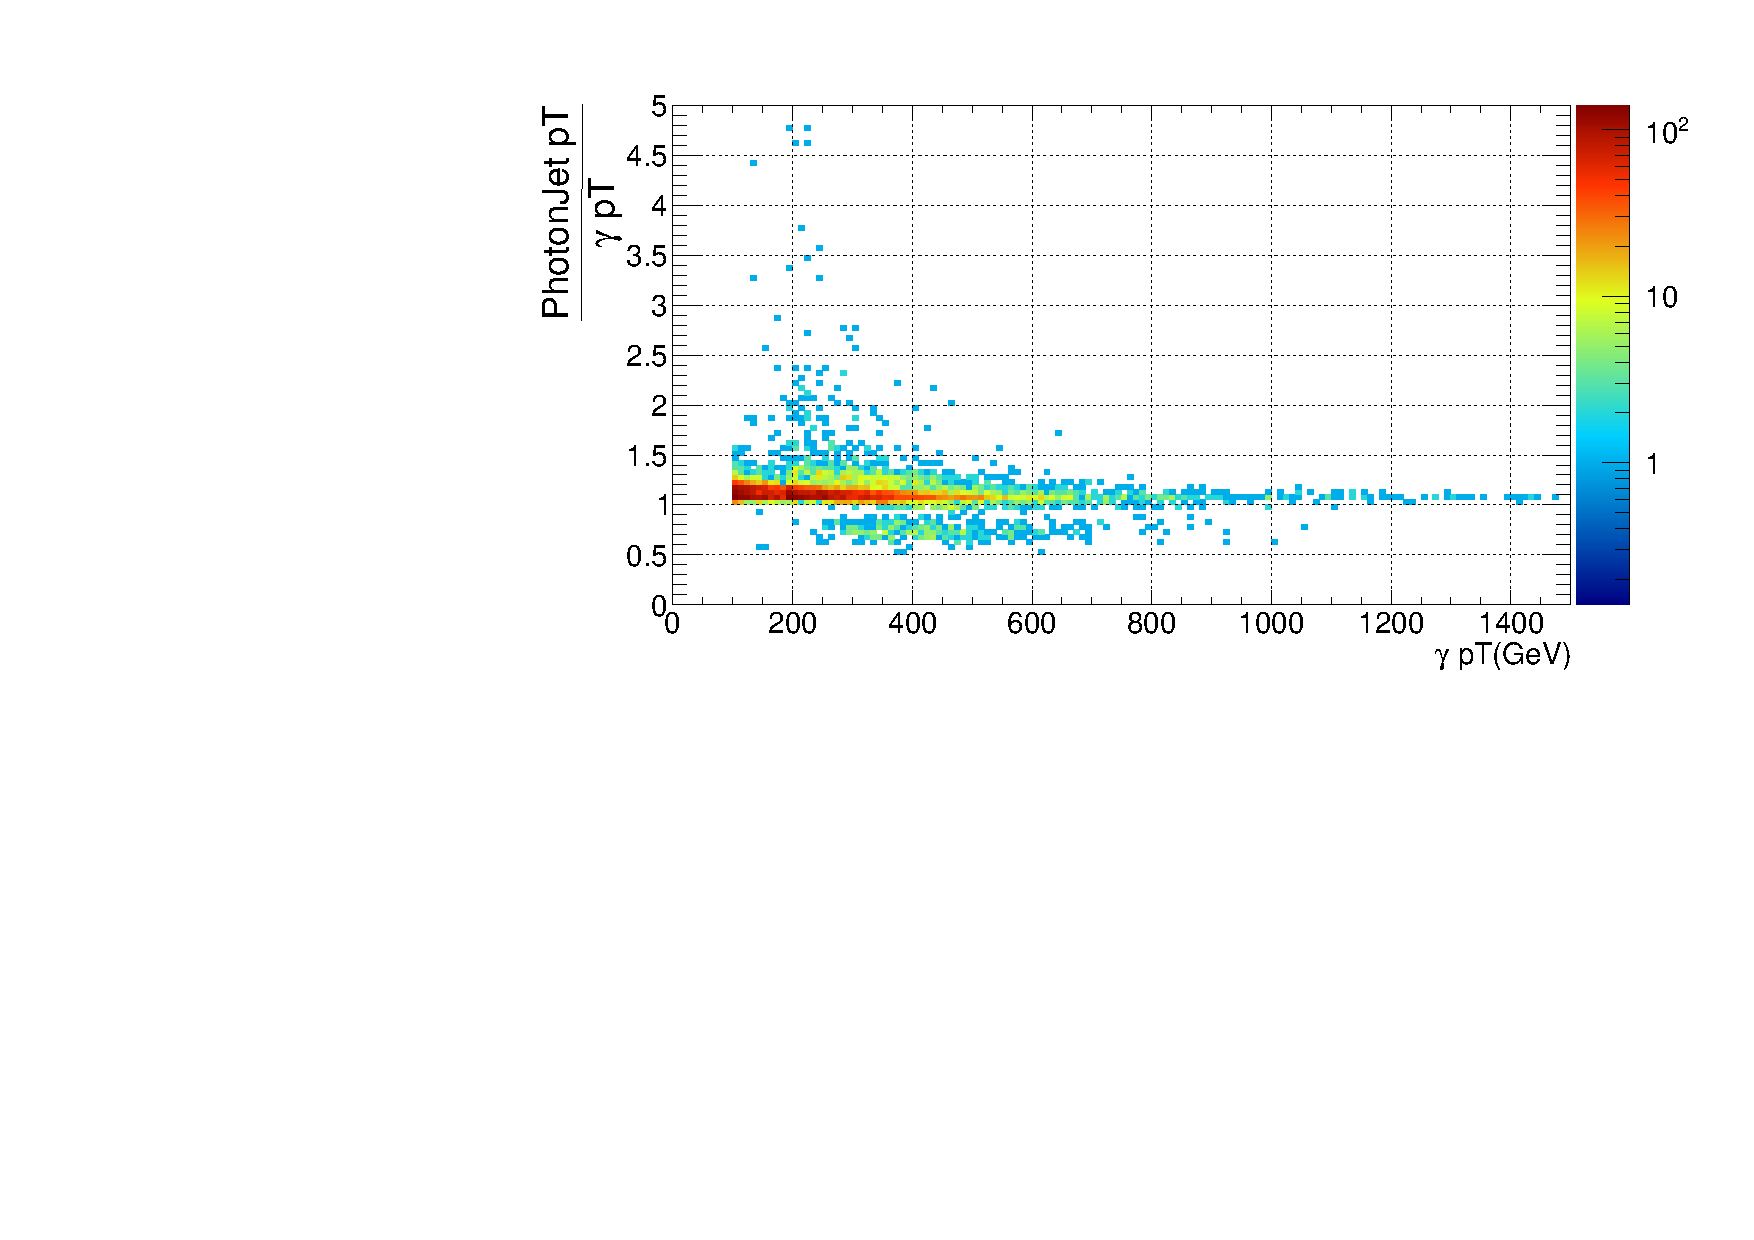
\includegraphics[width=0.48\linewidth]{../Figures/Chap2/appendix/RatioPhoJetPtToPhoPtVsPhoPt_AB_data.pdf}
  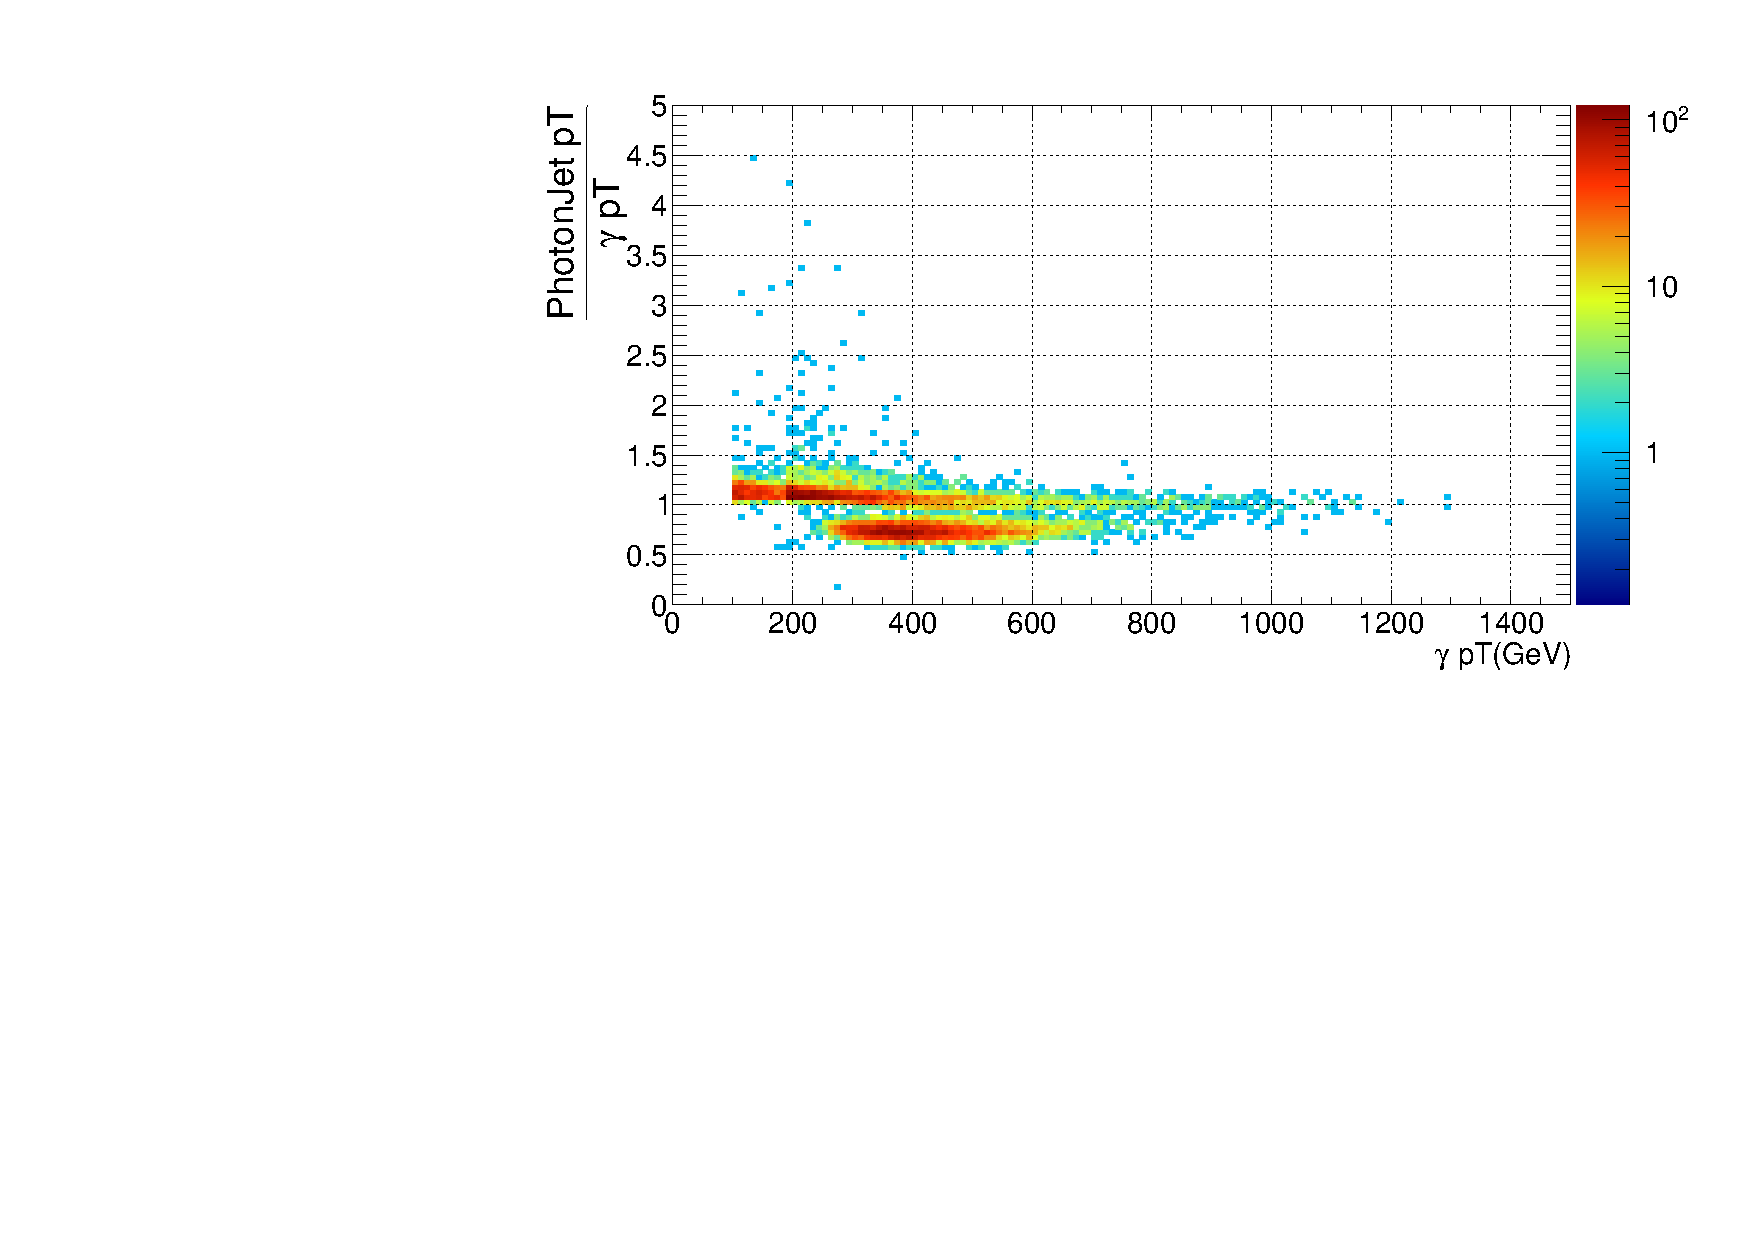
\includegraphics[width=0.48\linewidth]{../Figures/Chap2/appendix/RatioPhoJetPtToPhoPtVsPhoPt_C_data.pdf}
  \caption[Data cleaning]{Left column: $p_{\text{T}}^{jet}$/\ptg as a function of \ptg in low-\dphi region with $\ptmiss>100$~\gev region for events in \gjets events in MC (top-left) and for data (bottom-left). Right column: same quantities in high-\dphi region with $100<\ptmiss<200$~\gev for \gjets events in MC (top-right) and for data (bottom-right). }
  \label{fig:ratioVsPhotonPt}
\end{figure}